\chapter{Background}
% Add maximum likelihood background explanation
% Add Bayesian probability background explanation

\section{Computer Based Tests}
CBT abbreviation
- offers advantages such as being able to display higher quality visuals such as pictures, videos, graphs, etc...
- low paperwork, everything is stored on the computer
- automatic grading, less work for teachers
- generation of statistics is made easier by the fact that the data can be processed by the computer
- nowadays a lot of learning is done on computer systems, and children are used to dealing with computers so assessment through this medium is advantageous. \newline

CBTs are typically "fixed-item" tests where all the students answer the same set of questions,  usually provided by the person responsible for the assessment. This isn't ideal since students can be presented with questions that are too easy or too difficult for them to answer. Consequently, the results of the test won't give a very accurate representation of a student's ability, and for this reason, these types of tests aren't extremely useful. This problem lead to research and the development of computerized adaptive testing (CAT).

\section{Computerized Adaptive Testing}
Computerized adaptive testing (CAT), also called \textit{tailored testing}, is a form of computer-based testing which administers questions (referred to as \textit{items} in the psychometrics literature) of the appropriate difficulty by adapting to the examinee's ability.
For example, if an examinee answers an item correctly, then the next item presented will higher on the difficulty scale. On the other hand, if they answer incorrectly, they will be presented with an item lower on the difficulty scale. \newline

From an architectural perspective, a computerized adaptive test (CAT) consists of five components \cite{CAT-Framework}:

\subsubsection{1. Calibrated item pool}
An item pool is needed to store all the items available for inclusion in a test. This item pool must be calibrated with a psychometric model. During this phase, the item parameters are estimated according to the chosen model and scaled to fit with already existing items. Usually, the psychometric model employed in these systems is called Item Response Theory(IRT) (Section \ref{subsec:IRT}). Calibration is a complex process, and to be done accurately it requires a considerable amount of data. Typically, it is performed by psychometricians, aided by expensive and sophisticated calibration software.

\subsubsection{2. Starting point}
Initially, when zero items have been administered, no information is known about the examinees and so the CAT is unable to estimate their ability. As a result, the item selection algorithm will fail to choose the next item to be administered.
If there is previous information available, for example an examinee's ability estimate in a closely related subject, then this can be input into the system to form the starting point configuration. Often this data isn't available or too costly to collect, so the CAT's initial ability estimate for the examinee corresponds to the mean on the ability scale - hence the first item presented will be of average difficulty.

\subsubsection{3. Item selection algorithm}
The item selection algorithm chooses the next item to present to the examinee based on the ability estimate of the examinee up to that point.

There are several methods available to serve as the item selection algorithm, these will be examined when we consider IRT(section...)

\subsubsection{4. Scoring algorithm}
After an examinee has answered an item, the CAT will update its estim

\subsubsection{5. Termination criterion}

The CAT shouldn't be terminated too early, so as to allow enough time to estimate the examinee's ability with reasonable accuracy.

\begin{figure}[H]
\centering
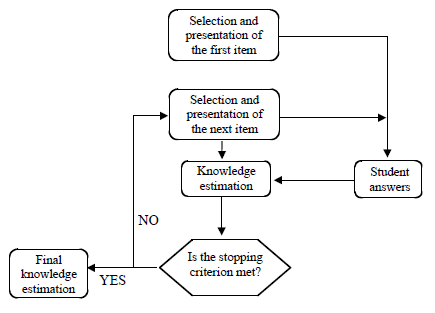
\includegraphics[scale=1]{cat_flowchart}
\caption{Flowchart of an adaptive test. Adapted from \cite{SIETTE}.}
\label{fig:cat_flowchart}
\end{figure}

The flowchart in figure~\ref{fig:cat_flowchart} corresponds to components 2-5, and illustrates the basics of the algorithm implemented in CAT. \cite{CAT-Wiki} gives a more detailed description of the procedure:
\begin{itemize}
\item[1.] The pool of items that haven't been administered yet is searched to determine the best item to present to the examinee, according to the current estimation of his ability.
\item[2.] The chosen item is presented to the examinee, who then answers it correctly or incorrectly.
\item[3.] The ability estimate is updated, based upon this new piece of information and the previous ability estimate.
\item[4.] Steps 1–3 are repeated until a termination criterion is met.
\item[5.] The algorithm returns a final ability estimate for the examinee's performance along with a confidence level: a percentage value indicating how accurate the estimate is.
\end{itemize}

CATs offer several advantages when compared to CBTs. As a result CATs have been used in many areas, ranging from education, hospital questionnaires, etc..

Advantages include
- precise scores for most test takers
- requires less items to be administered before arriving at an equally accurate score, in comparison to static multiple choice tests
- like any computer based test adaptive tests may show results immediately after testing, no grading having to be done by teachers, so saves time and money.

CATs present many attractive features but they do present a few disadvantages.
- the need for a large bank of calibrated items to cater to all ability levels.
- Items are administered one by one, so once an answer to the item has been given there is no turning back. No skipping questions either.

A brief overview of CATs was given in this section. All of these concepts will make more sense after reading the section on IRT and the implementation of adaptive testing in our system, jSCAPE.

\section{Probabilistic Test Theory}
\subsection{Maximum Likelihood}
% Add maximum likelihood background explanation
% Conditional probability quick overview?
% Add Bayesian probability background explanation
% Bayesian networks
% Latent variables ?

IRT is based on the idea that the probability of a correct/keyed response to an item is a mathematical function of person and item parameters. 

\begin{itemize}
\item Calculates the probability of a particular student answering a specific item correctly.
\item Different IRT models: One-Parameter Logistic (1-PL), Two-Parameter Logistic (2-PL), Three-Parameter Logistic (3-PL). Refers to the number of parameters used in the model. Parameters are: 

\begin{itemize}
\item[-] item difficulty parameter (\textit{b})
\item[-] item discrimination parameter (\textit{a})
\item[-] chance/guessing parameter (\textit{c})
\end{itemize}

\item Item Characteristic Curve, i.e. probability distribution
\end{itemize}

\subsection{Bayes probability theory}

\subsection{Item Response Theory}
\label{subsec:IRT}
For these reasons, Item response theory (IRT) has seen frequent usage when it comes to CATs....We present the different models developed to predict the probability of a correct or incorrect response to a particular item.
\subsubsection{The one-parameter logistic model}
dfsdfsdf
\subsubsection{The two-parameter logistic model}
dfsdfsdf
\subsubsection{The three-parameter logistic model}
dfsdfsdf
